\section{Experiments on finite-aperture scattering data}\label{sec:experiments}
\subsection{Materials, acquisitions and comparisons}
We count distinct simulated media and distinct laboratory objects. There are 72, plus a separate observation with two disjoint feasible material explanations. Table~\ref{tab:cohort} shows the role of each family. An acquisition at another frequency or with a different number of ports remains a paired observation. Previously examined objects are identified as such. The eight prospective pool targets were first generated after the weights, comparison arms, stopping rules and metrics were fixed. A ground-truth contrast or material mask was never used to rank a proposed region, select a reconstruction, or verify a lower bound. Declared supports in the compact tests are shared priors. The full-domain tests allow 9,216 independent parameters. Some contracts intentionally use identical forward and inverse grids to isolate an algebraic mechanism. Such a contract provides no continuum error estimate.

\begin{table}[!htbp]\centering\small
\caption{Distinct specimens contributing to each question. Array sizes are transmitters by receivers. These specimens contribute 120 registered acquisition views. A six-parameter ambiguity observation brings the total to 121. Two additional low-amplitude site controls reuse registered geometries.}\label{tab:cohort}
\begin{tabular}{@{}p{.33\linewidth}rp{.48\linewidth}@{}}\toprule
Material family & Number & Measurement and role\\\midrule
Large-domain, real & $6+22$ & $96^2$, $ka=11.85$, $10\times20$, 10\%. Six also at $32\times32$, 2\%.\\
Compact annular targets & 7 & $24^2$, $ka=4.27$, $12\times48$; cap 5 and data routing.\\
Loss-tangent geometries & 4 & $ka=3.55,7.40$, $10\times20$; three paired loss angles, 2\%.\\
Weak to moderate controls & $2+4$ & Two earlier shapes and four new shapes, first Born and full-wave data.\\
Chamber targets & $3+4$ & Fresnel at 4, 6, 8 GHz; Manitoba at seven frequencies from 3 to 6 GHz.\\
Structured sample pools & $4+8$ & Development and prospective samples respectively; $24^2$, $4\times16$, half aperture, 1.25\%.\\
Learned flow on its own geometry & 3 & $32^2$, signed contrast, two opposing sources, 16 receivers; 1\% tolerance.\\
Other mechanism controls & 5 & One $24^2$ annulus, one $32^2$ shape, one low-contrast disk, two site controls.\\\bottomrule
\end{tabular}
\end{table}

The large-domain synthetic measurements have physical frequency 400 MHz and a $2\,{\rm m}\times2\,{\rm m}$ field of view, with fixed total incident fluence within a paired comparison. The errors are joint complex Frobenius radii. We report a downward field-distance endpoint $d/r$ and, where available, a feasible point's upward endpoint. For inversion we report relative material $\ell^2$, target and background errors and held-out complex fields. Each comparator sees the same observations, geometry, masks and allowable material inputs within a comparison. The candidate-pool optimizer enforces its box throughout. The subsequent CIE comparison uses the actual contraction integral equation with its own state variables. Timings include proposals, full-wave solves, verification and unsuccessful attempts at the specified stage. Results on freshly simulated and previously archived measurements are distinguished.

\begin{figure}[!htbp]\centering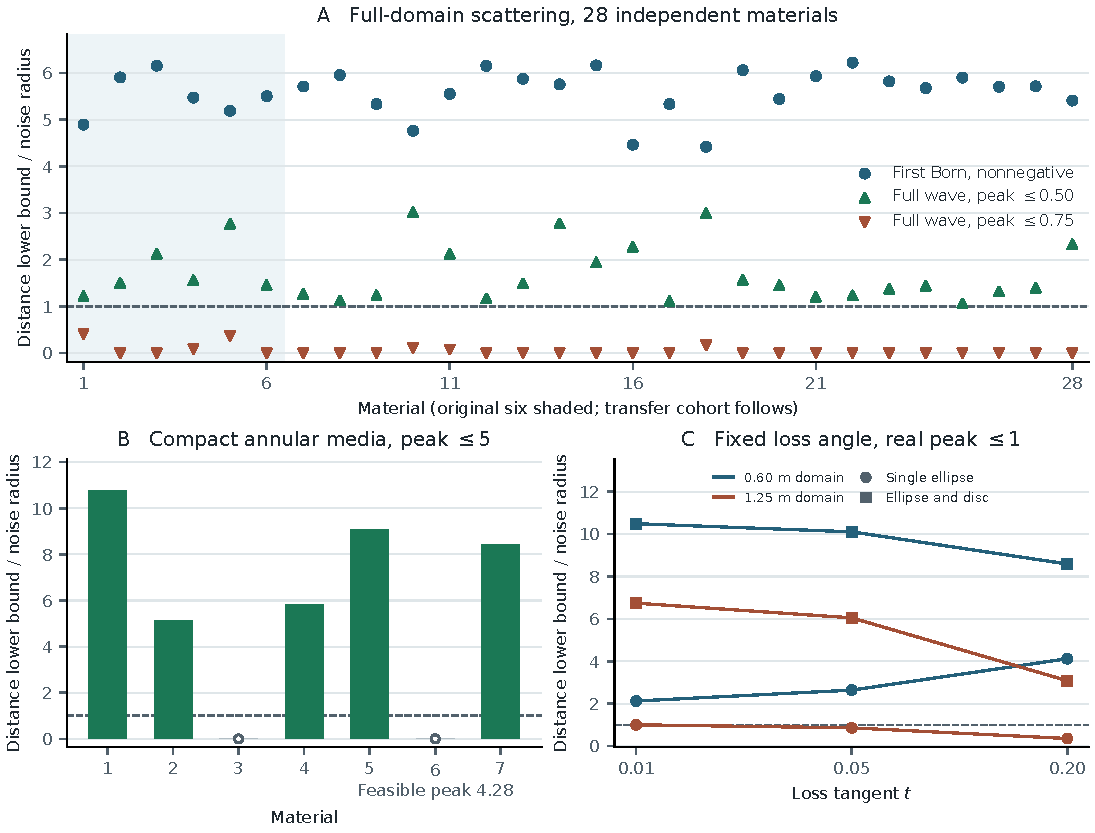
\includegraphics[width=.98\linewidth]{benchmark.pdf}
\caption{Bounds across every member of the primary lossless family and two other physical regimes. The reference line is the measurement error radius. Loss-angle comparisons use the same complex-material contract at each abscissa. Frequencies, hypotheses and noise levels are never counted as additional specimens.}\label{fig:benchmark}
\end{figure}

\subsection{From a blind contrast cap to a strong material neighbourhood}
On the primary 28 large-domain targets the nonnegative Born cone misses the receiver matrix by at least 43.88--61.94\% of its norm. At 10\% noise all 28 rule out the \emph{nonlinear} cap 0.50, with distances from $1.062r$ to $3.019r$. The same test at 0.75 excludes none. At 2\% noise with 32 sources and 32 receivers the six detailed cases give respectively five, three and one exclusions at 0.78125, 0.8125 and 0.84375, and none at one. Thus the strongest global statement on this six-target array remains that at least one cell of one target exceeds 0.84375. On seven distinct compact annular examples five exclude a cap of five. An admitted member of one of the other examples has peak 4.282. The difference in electrical area, illumination and measurement radius matters in comparing these regimes.

We next prescribe a high-valued material neighbourhood. Its circular support is fixed in each test, and its centre is either set by geometry or placed using only a Born adjoint of the readings. Contrast varies independently from cell to cell across an interval around a tapered profile. Vacuum outside the support gives an exact restriction of \eqref{eq:vie} to its active cells; all original ports remain. Table~\ref{tab:native} distinguishes a matched positive quadratic, a weaker material restriction and a physical point. A high-contrast class can be impossible for the simple reason that its support is wrong. On the first two 96² strong targets the lower endpoints removed at fixed support still give exclusions. On the 32² test that change instead leaves the comparison undecided. Two further experiments placed a known 78-cell dielectric of contrast 3.25 outside 437 uncertain cells, with the remaining 8,701 exterior cells fixed at vacuum. Including all interactions with this host gives lower bounds $29.00r$ and $27.73r$ under identity weighting, both with $\nu=7$ and 32 illuminations.

\begin{table}[!htbp]\centering\small
\caption{Same observations and supports, with nominal peak four. Columns show strict lower endpoints rounded down. The positive comparison is the best verified choice shown on the identical box; the final column relaxes the lower endpoints or supplies an admitted point. The asterisk marks an obstruction for the scalar spatial weights specified below.}\label{tab:native}
\begin{tabular}{lrrrrrp{.23\linewidth}}\toprule
Grid, object & Cells & $w$ & $\nu/s$ & $d/r$ & Pos. & Same support\\\midrule
$24^2$, annular & 177 & 2 & 2/12 & 57.37 & 54.74 & relaxed $>56.14r$\\
$32^2$, independent & 89 & 2 & 9/10 & 10.70 & 12.23 & relaxed $>0.43r$\\
$96^2$, slotted block & 749 & 2 & 9/32 & 18.94 & 25.05 & relaxed $>3.34r$\\
$96^2$, second target & 749 & 2 & 9/32 & 21.98 & 23.20 & relaxed $>6.27r$\\
$96^2$, disk & 1153 & 2.5 & 7/32 & 1.728 & $*$ & low peak fits within $0.99995r$\\\bottomrule
\end{tabular}
\end{table}

The disk provides a separation on \emph{one and the same support}. Its peak-0.625 reference satisfies the full-wave data within $0.999950r$. For the high branch the nominal peak is four; at the profile maximum the allowed interval is $[1.5,6.5]$. The strict lower endpoint is $1.7284581r$. A receiver-null unit vector has sector value at most $-0.22201567$ and radiation at most $1.4740\,10^{-17}$. It prevents positivity for every positive scalar sector multiplier with identity spatial weight and zero optical multiplier. For the recorded normalization the same conclusion holds for absolute optical-to-sector multiplier ratios below $1.5062\,10^{16}$. This is a limitation of those weights; general spatial reweighting is allowed by the theory.

For a tapered nominal profile $c_i$ the tested endpoints are $\max(0,c_i-w)$ and $c_i+w$. Thus $w$ is the nominal half-width; clipping acts only at the lower boundary. In this disk the norm contraction limit is bracketed by $[0.48604895,0.48604902]$. For the homogeneous upper perturbation in the box, $|\tr((wT)^4)|/1153>1.3932$ and hence $\rho(wT)>1.0864$. This makes the distinction stronger than failure of a sufficient contraction condition. The measured exclusion extends at least $5.1435$ times as far as its norm cutoff. At width $3.86436632$ the same low-peak physical witness belongs to the expanded box. The first possible fit is bracketed between $2.50$ (up to one binary rounding unit) and this latter width; its exact location is unknown. The proposal scan took 124.48 s wall and 125.04 s CPU across 241 boxes. The 22 main high-precision endpoint checks took 396.71 s wall and 583.71 s CPU. The extra radius and radiation analysis for the disk cost roughly 138 CPU s in addition to the high-box check. In particular this direct verification on a large support is a substantial additional calculation.

\begin{figure}[!htbp]\centering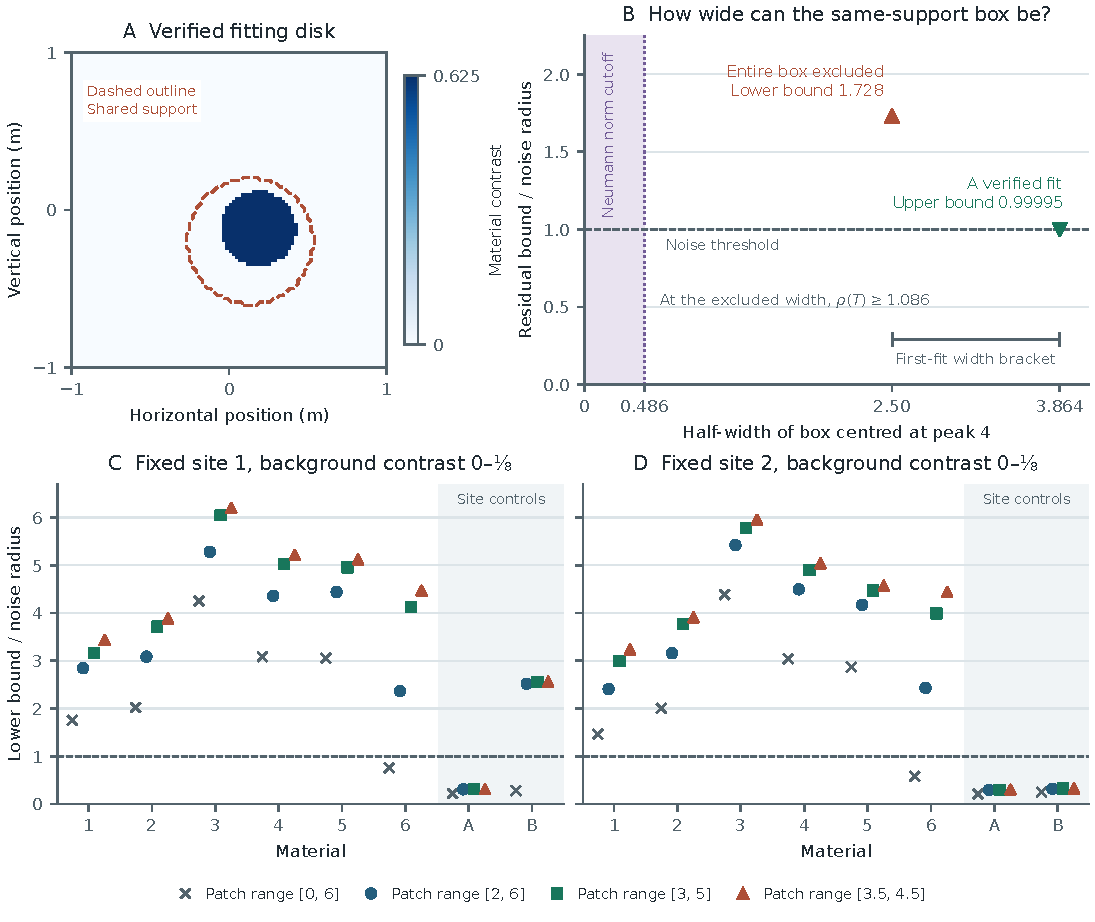
\includegraphics[width=.98\linewidth]{branches.pdf}
\caption{A high-contrast branch can be ruled out on a support that admits a different material. Allowing uncertainty in the entire exterior weakens the conclusion. The two-site comparison uses $8\times8$ candidate patches and the same array for eight receiver matrices.}\label{fig:branches}
\end{figure}

We relaxed the support assumption on the same 96² array. Two sites were specified in advance, each with $8\times8$ cells and independently variable contrasts. The other 9,152 cells now have arbitrary contrast in $[0,b]$. With nominal patch $[2,6]$ and $b=1/16$, both site hypotheses are excluded for each of the six detailed targets, with attained lower endpoints at least $7.89r$. Two additional compact controls of peaks 3.884 and 4.470 lie in their own site hypotheses, and the opposite site can be excluded in both. Doubling the background allowance to $1/8$ leaves only three of the six exclusions on both sites for the original matched weights. Transporting the parent $[0,6]$ weights using Proposition~\ref{th:transport} recovers all six at both sites, with lower endpoints from $2.36r$ to $5.42r$. This improves on directly reusing the broad-parent decision: the parent leaves one of the six unresolved on each site. For the two controls the wrong site is now excluded in one case ($d/r$ approximately 2.518), while the other is unresolved (approximately 0.496); both correct sites are retained. These endpoints use the better of two prespecified base multipliers $2^{-12}$ and $2^{-10}$. To isolate the role of the high lower endpoint, we generated a paired peak-0.625 amplitude on each of the same two patches. Both belong to the broad parent and fit their own readings within $0.999951r$. For these particular data the shifted $[2,6]$ child remains undecided even after weight transport: at $b=1/8$ the attained endpoints are $0.242r$ and $0.277r$. The comparison establishes an improvement across the six readings and exposes a remaining class of same-site ambiguities of the lower-bound test. The two new amplitudes are paired controls in addition to the registered acquisition views. Geometry work took $0.97+2.70+3.46$ s. The 32 original profiles and 256 readouts took 16.44 s including all choices. The transported comparison, repeating geometry and evaluating 24 profiles for eight readings each, took 17.27 s wall.

\subsection{What does a candidate pool buy?}
On four development objects a fixed data-driven proposal constructs sixteen overlapping boxes and four samples per box. All candidates share the same known $7\times7$ support on a $24^2$ physical grid; multi-source scattering within it is exact. The distinct objects have peaks from 3.99 to 4.60. The fit uses four illuminations and 16 of 32 receivers; disjoint receiver and illumination readings are reserved for scoring. For each box the same full-wave bound-constrained quasi-Newton solver can vary all 49 active materials for 42 function evaluations. The strong point comparator pays for full-wave propagation of all 64 samples, then refines boxes in order of point residual until the first verified fit. The exhaustive comparator refines all sixteen. Geometric support and unrestricted reciprocal current transfer can fit any of the measured port matrices on this patch (Appendix~\ref{app:tech}); material information is essential.

Conventional and source-directional Neumann bounds rule out four of 64 boxes. Replacing all positive lower endpoints by zero permits the sector computation to reject fourteen. The centred intervals eliminate forty, leaving respectively nine, six, five and four candidates. All eight boxes that actually cover their generating material survive. These eight are broad proposal priors; no narrow box in this development set covers its generator. Selecting only the best single sample misses a noise-ball fit on three of four objects. Refining in order of point fit instead reaches the tolerance after one or two boxes on every object. The complete interval procedure uses 1,154 optimization factorizations against 2,367 for exhaustive refinement, yet wall time rises from 0.082--0.111 s to 0.777--1.135 s per object. Point ranking followed by refinement takes 0.028--0.036 s. Exclusion of every member of a box and receipt of a single acceptable image have different costs.

To reduce that cost we used the bordered count at just one source threshold. On the four development objects it recovers all forty exclusions with at most two scalar weights. Before generating eight new target geometries, the weights, threshold, refinement allowance, sixteen proposal families and noise rule were fixed. Figure~\ref{fig:pools} shows all eight outcomes. Respectively 13, 12, 13, 12, 9, 14, 13 and 12 boxes were excluded. All ten truth-containing boxes survived. Every exclusion was independently enclosed by complex ball arithmetic. Seven objects yielded a verified physical fit with all three methods. On the remaining object the generator fits the noisy measurement, but the constrained optimizations exhausted their budgets. An unresolved or unvisited box was never classified as a physical branch.

\begin{table}[!htbp]\centering\small
\caption{Prospective 49-cell inversions, eight independent materials. Medians are per target. The fixed input error is 1.25\%. Receiver and illumination holdouts are scored independently. All three methods had seven accepted endpoints; the common failure is included in the error medians.}\label{tab:pool}
\setlength{\tabcolsep}{3pt}\begin{tabular}{@{}lrrrrr@{}}\toprule
Method & Wall (ms) & CPU (ms) & LU & Image & Rx / Tx\\\midrule
All sixteen boxes & 82.5 & 81.9 & 535.5 & 10.02\% & 1.16 / 1.67\%\\
Points until first fit & 37.1 & 37.0 & 183 & 10.02\% & 1.16 / 1.67\%\\
Test surviving boxes & 54.6 & 54.5 & 179.5 & 10.02\% & 1.16 / 1.67\%\\
\bottomrule\end{tabular}
\end{table}
The point-ranked arm stops after one or two boxes on seven targets. On the eighth, all sixteen fail to reach tolerance (74.6 ms and 577 LU). The bordered arm refines all two to seven survivors per target. On the eighth this takes 56.8 ms and 119 LU. On every target its best material comes from the broad initial prior box. The median independent interval replay took a further 362.7 ms per target and rechecked the 98 exclusion decisions. Table~\ref{tab:pool} includes the online floating-point error bounds and the endpoint forward checks. Including the additional replay gives roughly 0.42 s per object. Solver setup, proposals, ranking, field solves and endpoint checks were timed on the same Apple M4; rates need not carry over to another implementation.

To isolate the cost of a single image, we then gave both arms exactly the same stopping objective on these eight exposed targets. Both propagate all 64 points, refine the best sample of each ranked box, and stop at the first verified fit. One arm also screens boxes before refinement. In ten paired runs per target, both return identical materials on all eight; both find seven fits. Summing the eight per-target median times yields 0.258 s without screening and 0.296 s with screening. The latter uses 1,409 instead of 1,803 full-wave factorizations. All seven successful targets take longer when screened. On the common failure it skips fourteen boxes, reducing time from 57.65 to 34.61 ms and factorizations from 577 to 183. An independent replay of the 98 exclusions cost a further 2.137 s for the eight targets. Thus fewer field solves yield a time saving on the hard target, but not on this cohort overall.

\begin{figure}[!htbp]\centering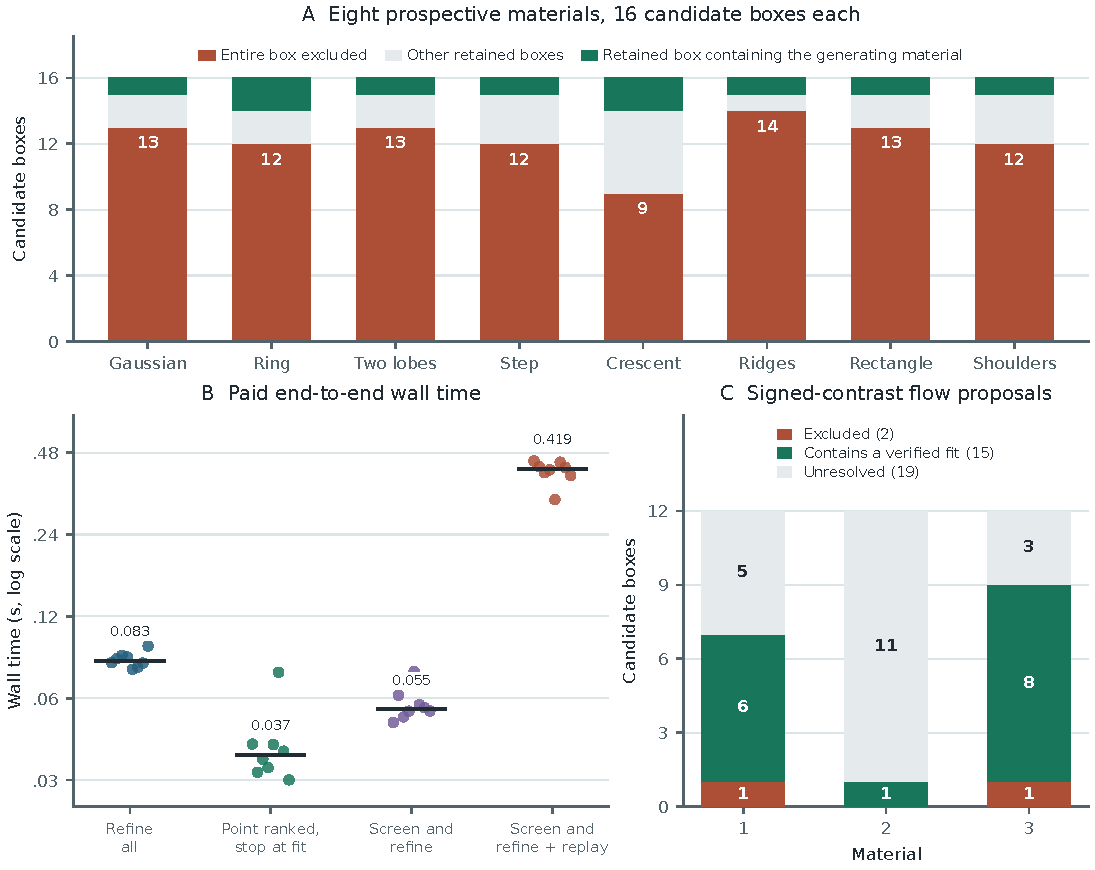
\includegraphics[width=.99\linewidth]{pools.pdf}
\caption{What is gained by testing whole material boxes? Paired prospective results show the number excluded and the time to an image. A separate learned generator uses its own signed material and aperture convention. Its boxes can contain physically feasible alternatives while missing the generating material.}\label{fig:pools}
\end{figure}

\paragraph{Same four comparisons with a current-domain inversion.}
We repeated the branch experiment using a hard-box contraction integral equation. All four arms use the same deterministic visible current, rank four, Fourier current updates at 4, 16 and 36 columns, two contraction parameters, a common source-wise conjugate-gradient update, and a shared contrast at each active cell. The contrast is projected into the proposed interval at every voxel readout. Settings were fixed before these current iterations; the twelve geometries had already been used in the preceding comparisons. The pure CIE schedule leaves \emph{all} twelve outside the discrepancy radius (best per case $1.668r$--$4.307r$). Although the box test avoids many iterations, this experiment alone does not demonstrate faster recovery.

We therefore followed each current-domain output by the same 42-evaluation box-constrained nonlinear corrector, with original-field acceptance. Table~\ref{tab:ciepool} includes the new calculation for all 12 objects. Every arm now gives a verified fit on every object. The interval arm returns the same materials as exhaustive refinement in each case. The online time falls from 4.96 s to 1.89 s. Including the independent 2.882 s ball-arithmetic replay of all 138 exclusions brings this to 4.775 s, close to the exhaustive 4.963 s. All eighteen truth-containing boxes survive. The more demanding comparison is the point-ranked arm, which stops at a fit and takes 0.89 s. The choice between eliminating material classes and returning a first compatible map remains observable even with a genuine current-space inversion and successful endpoints.
\begin{table}[!htbp]\centering\small
\caption{Paired, independently timed current-domain refinement followed by a physical corrector on 12 targets already exposed to the study. Wall and LU counts are totals. Image and withheld-port errors are reported in the text as medians. All 48 selected images fit their measurement balls. Independent ball-arithmetic replay adds 2.882 s to the bordered arm.}\label{tab:ciepool}
\begin{tabular}{@{}lrrrr@{}}\toprule
Material selection & Wall, s & CPU, s & Full-wave LU & Fits\\\midrule
All boxes & 4.963 & 4.878 & 8672 & 12/12\\
Point rank until fit & 0.890 & 0.873 & 2430 & 12/12\\
Neumann survivors & 6.456 & 6.331 & 8464 & 12/12\\
Bordered-test survivors & 1.892 & 1.866 & 3516 & 12/12\\\bottomrule
\end{tabular}
\end{table}
The interval arm has median material error 6.71\%, held-out receiver error 0.978\% and held-out illumination error 1.407\%. Point ranking yields 6.42\%, 1.108\% and 1.370\%. At the 42-evaluation allowance, direct point-ranked physical optimization without CIE missed one object ($1.042r$). In a follow-up restricted to that exposed failure, doubling the direct allowance yields a verified $0.9531r$ at the second ranked box in 0.041--0.042 s. The CIE and corrector point arm on that object used 0.071 s. This check removes the apparent necessity of the CIE start. No target was replaced after the initial failure.

A learned flow was evaluated on its original $32^2$ signed-contrast model with two opposing incident waves and 16 observed receivers. We regenerated 64 samples per object using the stored weights, formed twelve Ward clusters and expanded each coordinate range by 0.10. This experiment uses three previously exposed held-out materials and clean archived readings with a 1\% tolerance. Their generating materials are outside \emph{all} 36 boxes. After 39 budgeted full-wave evaluations per cluster, verified physical materials enter six, one and eight boxes respectively. Best point residuals are $0.276r$, $0.937r$, $0.470r$, with material errors 26.35, 79.36 and 51.53\% despite held-out receiver errors below 1\%. The signed sector excludes two further boxes at $3.294r$ and $8.455r$, both with positive state curvature and perturbation norm at most 0.52. The standard Neumann distance and tested directional bounds reject neither. Across the three readings, fifteen boxes admit verified physical points, two are excluded and nineteen remain unresolved. Across two objects, 25 pairs of disjoint boxes contain verified alternatives. The original generating materials were independently accepted in their own data balls. Verified lower bounds for the diameter of the material feasible set are 26.35, 79.36 and 51.53\% of the respective generating norms. The sector search and verification here take about 34 s for the three readings, including about 13 s for the 36 proposals and 21.36 s for independent ball-arithmetic checks and their shared setup. Point ranking to the first fit reaches cluster ranks one, seven and one, with stage-summed totals of 7.21, 11.91 and 4.55 s. The corresponding box-first totals are 29.87, 21.50 and 27.72 s; exhaustive refinement takes 19.37, 17.50 and 17.01 s. An observation with two much more widely separated materials at an extremely small tolerance gives a useful counterexample to always selecting one branch: Appendix~\ref{app:tech} reports both directly checked physical endpoints.

Figure~\ref{fig:maps} shows the selected fields on a common contrast scale. The low residual in the last row is consistent with the observed receiver matrix even when the image visibly differs from the generating material.
\begin{figure}[!htbp]\centering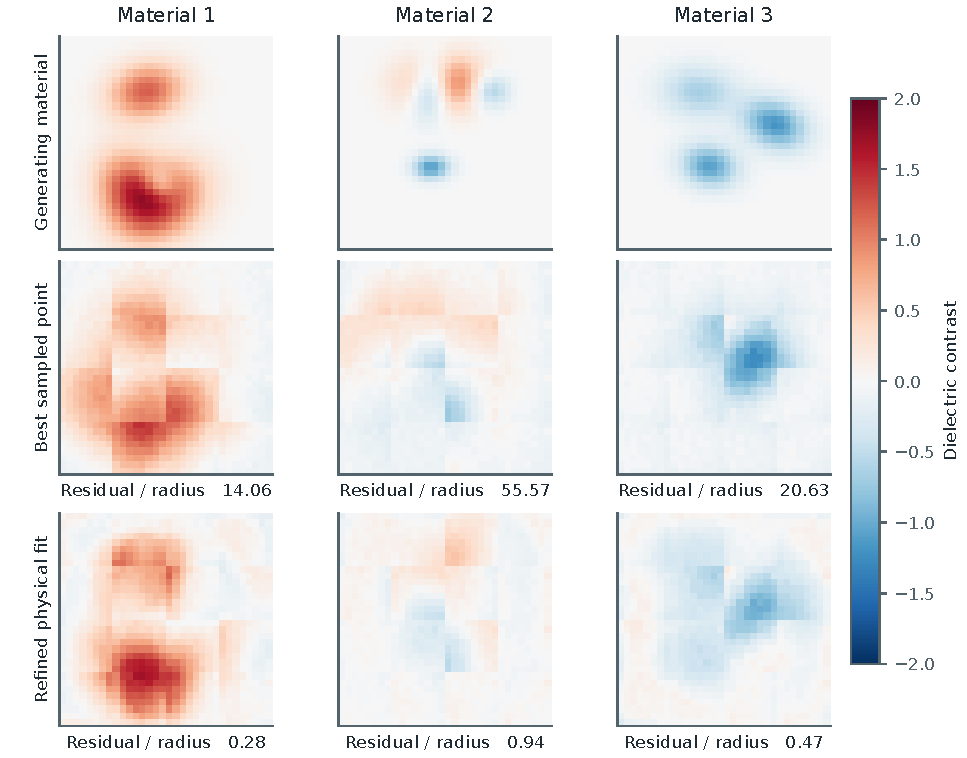
\includegraphics[width=.83\linewidth]{material-alternatives.pdf}
\caption{Three signed-contrast materials and alternatives proposed from two incident waves. Middle row: the best of 64 original samples by full-wave data misfit. Bottom row: the best full-wave fit from the twelve refined material boxes. Selection uses the measured receiver data alone; the top row is revealed for scoring.}\label{fig:maps}
\end{figure}

\subsection{Does the decision improve nonlinear reconstruction?}
On the 28 primary targets, the Born decision took a median 0.142 ms after 0.269 s of geometry preparation. Its rejected images still supply useful initial guesses. With the same $[0,4]$ box, 24² grouped material updates on the native forward grid and sixteen objective evaluations, Born initialization improves the training residual on 15 of 28 targets and the material error on ten. One example changes from $9.825r$ to $4.662r$ and from 0.996 to 0.870 in relative material error. No endpoint in either arm on these targets attains the error radius. A routed zero initialization costs 106.61 s summed over the 28 objects, versus 108.15 s with a Born start. On four new weak-to-moderate geometries Born initialization improves all four final material and residual errors, although two fail the linear terminal test. The test detects a physical failure of the linear model; it does not select an optimal solver.

Matching the material box in a native contraction integral-equation method gives 32.30 and 32.72 s for 28 vacuum and Born starts. At 16 current steps the median material errors are 0.913 and 0.919, inside-target errors 0.686 and 0.682, background RMS 0.674 and 0.686, held-out field errors 1.100 and 1.107. Independent full-wave residuals are $10.46r$ and $10.61r$. Two longer three-stage runs still ended above $8r$ after 96 steps. These are capped optimization comparisons. They do not establish a lower bound on the performance of a converged CIE or SOM solve.

On the slotted block and staggered grooves at 2\% noise, the 13-dimensional negative current projection must have norm above 15.76 and 19.76 respectively for any fit at peak at most one. The ordinary 100-column Fourier basis already meets this space at principal angles of $0.91$--$5.47$ degrees. We replace thirteen columns by orthogonalized negative modes at fixed basis width, measured aperture, deterministic-current rank, and iteration count. Relative image errors improve from 0.959 to 0.922 and 0.819 to 0.779, but training residuals worsen from $59.66r$ to $60.45r$ and $53.31r$ to $53.80r$; held-out complex fields worsen on both. The necessary norm is met by all four peak-clipped points, whose field discrepancies exceed $65r$. Directly pulling back the bordered inequality to the actual affine subspaces also rules out neither basis. A fixed contraction parameter of two accounts for much of the early reduction obtained by a peak-informed choice. A larger necessary norm supplies no quantitative independent gain in image recovery in these comparisons.

Finally, two full-domain CIE iterates were tested with actual local boxes. With half-width 0.04 both the new and perturbative bounds were undecided. Narrowing to 0.005 gave $7.970r$ and $17.952r$; the analogous Neumann bounds already gave $5.599r$ and $16.353r$. All restart policies chose the same continuation. Ordinary unconfined continuation left the two narrow boxes in respectively 94 and 140 pixels. This directly checks the premise needed for interpreting a local box as a basin. The box proof added 0.67--0.79 s.

\subsection{What changes with losses and laboratory measurements?}
On four distinct positive loss-tangent geometries, with $t_\ell=0.01,0.05,0.20$ paired within each, all twelve known-phase Born cones can be excluded. The compact example at $t_\ell=0.05,u=0.75$ illustrates what dissipation contributes under the same physical assumptions. Every common scalar energy multiplier gives less than $0.80975r$; applying the same law with separate weights in coherent source directions gives more than $1.01323r$, and the full receiver ellipsoid more than $1.02003r$. At $u=1.25$ one compact example gains from jointly using the absolute material sector and the dissipative information in distinct illumination directions. The larger examples can remain inside the relaxed receiver ellipsoid. Their undetermined peaks cannot be assigned the bound from a different loss tangent.

Real measurements from the Fresnel and Manitoba facilities \cite{fresnel,manitoba} delimit the error interpretation. Born distances exceed the reported reference error scales in three of nine and 25 of 28 frequency views respectively. No Fresnel view at cap 0.5 clears the held-out empty-scene scale. At passive cap one, the large Manitoba nylon cylinder at 3 GHz leaves 4.018\% of the field norm for further loaded-scene error after accounting for calibration spread. In separate training-only Born fits, relative receiver holdout errors range from 80.2 to 97.9\% at Fresnel and from 68.1 to 107.9\% at Manitoba; separate source holdout errors are 91.4--116.8\% and 69.0--104.8\%. A loaded-scene forward error below the quoted headroom has not been established. The chamber data therefore support a conditional error budget and an independent field prediction comparison.
